\documentclass[border=6pt]{standalone}
\usepackage[T1]{fontenc}
\usepackage{courier}
\usepackage[scaled=0.95]{helvet}
\renewcommand{\familydefault}{\sfdefault}
\usepackage{sfmath}
\usepackage[version=4]{mhchem}
\usepackage{tikz}
\usepackage{pgfplots}
\pgfplotsset{compat=newest}
\usetikzlibrary{arrows.meta,positioning,calc,fit,backgrounds,shapes.geometric,decorations.pathreplacing,patterns}
\definecolor{ink}{HTML}{17233A}
\definecolor{inksoft}{HTML}{44506A}
\definecolor{teal}{HTML}{0E6B6B}
\definecolor{tealsoft}{HTML}{E5F0EF}
\definecolor{amber}{HTML}{B26B12}
\definecolor{ambersoft}{HTML}{FBF0DF}
\definecolor{blue}{HTML}{2F6690}
\definecolor{bluesoft}{HTML}{E3ECF4}
\definecolor{plum}{HTML}{7A4D8C}
\definecolor{plumsoft}{HTML}{EFE7F3}
\definecolor{greyc}{HTML}{8A94A3}
\definecolor{linec}{HTML}{D3DCE1}
\definecolor{oxy}{HTML}{C0392B}
\definecolor{carb}{HTML}{3B4252}
\definecolor{hyd}{HTML}{E6E9EE}
\definecolor{nit}{HTML}{2F6690}
\tikzset{
  every picture/.style={line cap=round,line join=round},
  lab/.style={font=\small, text=inksoft},
  >={Stealth[length=7pt]},
}
\pgfplotsset{
  every axis/.append style={axis line style={inksoft}, tick style={inksoft}, tick label style={font=\footnotesize, text=inksoft}, label style={font=\small, text=ink}},
}
% fragment tile: \frag{node name}{position}{colour}{content}
\newcommand{\frag}[4]{\node[draw=#3, fill=#3!12, line width=1.4pt, rounded corners=6pt, minimum width=1.25cm, minimum height=1.05cm, text=#3, font=\bfseries] (#1) at (#2) {#4};}
\newcommand{\ring}{\tikz[baseline=-0.6ex]{\draw[line width=1.1pt] (0:0.3)--(60:0.3)--(120:0.3)--(180:0.3)--(240:0.3)--(300:0.3)--cycle; \draw[line width=0.8pt] (0,0) circle (0.16);}}
\newcommand{\bond}[2]{\draw[ink, line width=2.2pt] (#1) -- (#2);}

\begin{document}
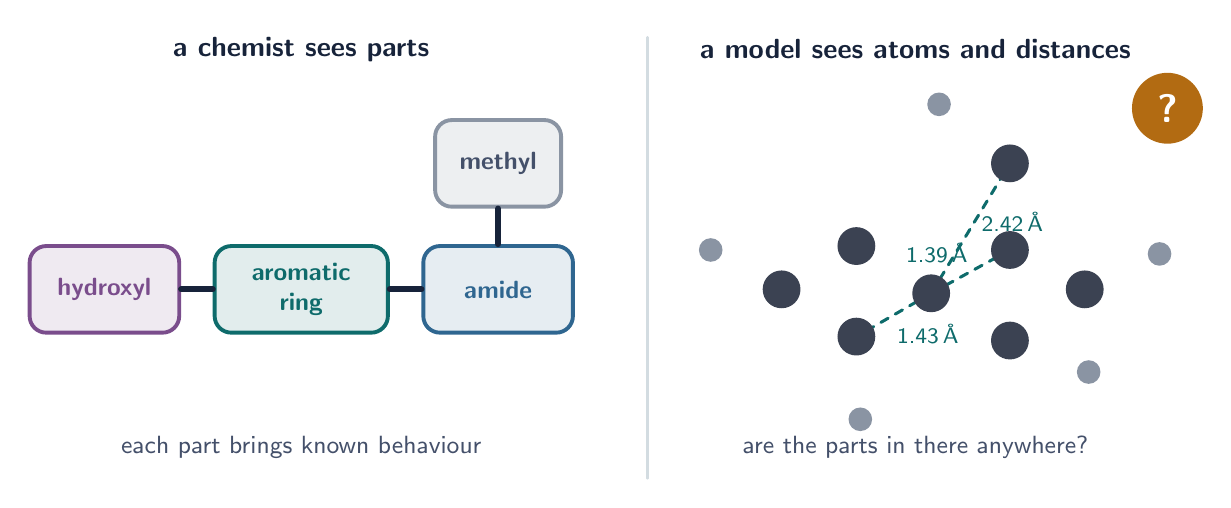
\begin{tikzpicture}
\node[font=\bfseries, text=ink] at (2.6,4.45) {a chemist sees parts};
\node[draw=teal, fill=teal!12, line width=1.4pt, rounded corners=6pt, minimum width=2.2cm, minimum height=1.1cm, text=teal, font=\bfseries\small, align=center] (r) at (2.6,1.4) {aromatic\\ring};
\node[draw=blue, fill=blue!12, line width=1.4pt, rounded corners=6pt, minimum width=1.9cm, minimum height=1.1cm, text=blue, font=\bfseries\small] (am) at (5.1,1.4) {amide};
\node[draw=plum, fill=plum!12, line width=1.4pt, rounded corners=6pt, minimum width=1.9cm, minimum height=1.1cm, text=plum, font=\bfseries\small] (oh) at (0.1,1.4) {hydroxyl};
\node[draw=greyc, fill=greyc!15, line width=1.4pt, rounded corners=6pt, minimum width=1.6cm, minimum height=1.1cm, text=inksoft, font=\bfseries\small] (me) at (5.1,3.0) {methyl};
\bond{oh}{r}\bond{r}{am}\bond{am}{me}
\node[font=\small, text=inksoft, align=center] at (2.6,-0.6) {each part brings known behaviour};
\draw[linec, line width=1pt] (7.0,-1.0) -- (7.0,4.6);
\node[font=\bfseries, text=ink] at (10.4,4.45) {a model sees atoms and distances};
\draw[teal, line width=1.1pt, dashed] (10.60,1.35) -- (11.60,1.90) node[pos=0.55, above left, font=\footnotesize, text=teal, inner sep=2pt] {1.39\,\AA};
\draw[teal, line width=1.1pt, dashed] (10.60,1.35) -- (9.65,0.80) node[pos=0.55, below right, font=\footnotesize, text=teal, inner sep=2pt] {1.43\,\AA};
\draw[teal, line width=1.1pt, dashed] (10.60,1.35) -- (11.60,3.00) node[pos=0.55, right, font=\footnotesize, text=teal, inner sep=2pt] {2.42\,\AA};
\fill[carb] (10.60,1.35) circle (0.24);
\fill[carb] (11.60,1.90) circle (0.24);
\fill[carb] (12.55,1.40) circle (0.24);
\fill[carb] (11.60,3.00) circle (0.24);
\fill[carb] (9.65,1.95) circle (0.24);
\fill[carb] (8.70,1.40) circle (0.24);
\fill[carb] (9.65,0.80) circle (0.24);
\fill[carb] (11.60,0.75) circle (0.24);
\fill[greyc] (13.50,1.85) circle (0.15);
\fill[greyc] (10.70,3.75) circle (0.15);
\fill[greyc] (7.80,1.90) circle (0.15);
\fill[greyc] (9.70,-0.25) circle (0.15);
\fill[greyc] (12.60,0.35) circle (0.15);
\node[circle, fill=amber, text=white, font=\Large\bfseries, minimum size=0.9cm] at (13.6,3.7) {?};
\node[font=\small, text=inksoft, align=center] at (10.4,-0.6) {are the parts in there anywhere?};
\end{tikzpicture}
\end{document}
